\documentclass{article}
\usepackage[T1]{fontenc}
\usepackage{lmodern}
\usepackage{graphicx}
\usepackage{amsmath,amssymb}
\usepackage[a4paper,margin=2cm]{geometry}
\usepackage[absolute,overlay]{textpos}
\setlength{\TPHorizModule}{1mm}
\setlength{\TPVertModule}{1mm}
\usepackage[indonesian]{babel}
\usepackage{hyperref}
\setlength{\emergencystretch}{2em}
% unit: Halaman 5

\begin{document}

% === Halaman 5 (llm) ===

\section*{Gilbert Vernam}

\vspace{139.89mm}

From Wikipedia, the free encyclopedia

\textbf{Gilbert Sandford Vernam} (April 3, 1890 -- February 7, 1960) was a Worcester Polytechnic Institute 1914 graduate and AT\&T Bell Labs engineer who, in 1917, invented an additive polyalphabetic stream cipher and later co-invented an automated one-time pad cipher. Vernam proposed a teleprinter cipher in which a previously prepared key, kept on paper tape, is combined character by character with the plaintext message to produce the ciphertext. To decipher the ciphertext, the same key would be again combined character by character, producing the plaintext. Vernam later worked for the Postal Telegraph Company, and became an employee of Western Union when that company acquired Postal in 1943. His later work was largely with automatic switching systems for telegraph networks.

\vspace{10mm}

\begin{tabular}{|l|l|}
\hline
\multicolumn{2}{|c|}{\textbf{Gilbert Vernam}} \\ \hline
\textbf{Born} & April 3, 1890 \\ \hline
\textbf{Died} & February 7, 1960 (aged 69) \\ \hline
\textbf{Alma mater} & Worcester Polytechnic Institute \\ \hline
\textbf{Occupation} & Cryptographer \\ \hline
\end{tabular}

% deskripsi: Foto potret hitam putih Gilbert Vernam
% bbox normalisasi: [0.7700, 0.2030, 0.9520, 0.6740]
\begin{textblock*}{38.22mm}(161.70mm,60.29mm)
\noindent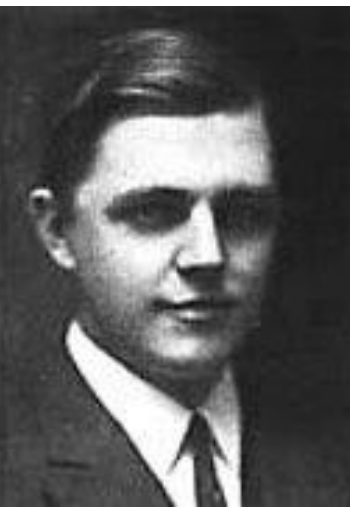
\includegraphics[width=38.22mm,height=139.89mm]{../../images/llm/page_005_img_01.png}%
\end{textblock*}

\end{document}
